\documentclass[supercite]{HustGraduPaper}
%进行个人信息设置
\title{RIS辅助的无线通信系统的原型验证} %论文题目
\author{裴熙隆} %作者姓名
\date{\today} %日期,默认当日
\school{人工智能与自动化学院} %院系名称
\classnum{自动化1705班} %专业班级
\stunum {U201714286} %学号
\instructor{陈忠、尹海帆} %指导教师姓名

%添加自己要用的其他宏包
\usepackage{xltxtra}
\usepackage{bm}
\usepackage{array}
\usepackage{multirow}
\usepackage[caption=false,font=footnotesize]{subfig}
\usepackage{algorithm}
\usepackage{algorithmic}

\begin{document}
%生成标题页 \maketitle[可选参数]\end{document}\end{document}
%可选参数:
%logo color=green/black 华中科技大学字样的颜色,绿色或者黑色,默认绿色
%line length=12em 填写信息处横线的长度,默认12em
%line font=huawenzhongsong 填写信息的字体,默认huawenzhongsong
\maketitle

%生成声明与授权书页 \statement[可选参数]
%可选参数:
%confidentiality=yes/no/true/false/empty
%是否保密,yes/true为保密;no/false为不保密,empty为不填,默认为empty
%year=5 保密年数,默认为空
\statement[confidentiality = false]

\clearpage %结束上一页
\pagenumbering{Roman} %摘要页码为大写罗马数字

%填写中文摘要内容和关键字
\begin{cnabstract}{可重构智能表面;智能反射面;无线中继;大规模多进多出系统;原型系统;现场可编程逻辑门阵列}
	%请注意使用中文分号“;”分割关键词!

	近年来,

\end{cnabstract}
%填写英文摘要内容和关键字
\begin{enabstract}{Reconfigurable intelligent surface; intelligent reflecting surface; wireless repeating; massive multiple-input multiple-output; prototype; field programmable gate array}
	%Please Use English Semicolon and a Space "; " to Separate Keys! 

	Recently,

\end{enabstract}

%生成目录 \tableofcontents[可选参数]
%可选参数:
%pagenum=yes/no/true/false 目录是否显示页码,默认为false
%toc in toc=yes/no/true/false 目录中是否有目录及其页码,默认为false
%level=4 目录级数,默认是4,即显示到subsubsubsection
%section indent=0em 目录第一级的缩进,默认是0em
%subsection indent=1.5em 目录第二级的缩进,默认是1.5em
%subsubsection indent=3.8em 目录第三级的缩进,默认是3.8em
%subsubsubsection indent=7em 目录第四级的缩进,默认是7em
%paragraph indent=11em 目录第五级的缩进,默认是11em
%subparagraph indent=13em 目录第六级的缩进,默认13em
%indent=normal/noindent/hustnoindent/sameforsubandsubsub 快速缩进设置,具体见文档
%dot sep=4.5 目录点间距,默认4.5
%section dot sep=4.5 目录第一级的点间距,默认是4.5
%subsection dot sep=4.5 目录第二级的点间距,默认是4.5
%subsubsection dot sep=4.5 目录第三级的点间距,默认是4.5
%subsubsubsection dot sep=4.5 目录第四级的点间距,默认是4.5
%paragraph dot sep=4.5 目录第五级的点间距,默认是4.5
%subparagraph dot sep=4.6 目录第六级的点间距,默认是4.5
%请注意在合适的位置放置\pagenumbering{numstyle}使用新的页码
\tableofcontents

\clearpage%结束上一页
\pagenumbering{arabic} %正文页码为阿拉伯数字

%正文内容从这里开始
\section{绪论}
%这是小四号的正文字体,段间距1.5倍
%通过空一行实现段落换行,仅仅是回车并不会产生新的段落
%\par 也可以通过\verb|\par|命令来新起一段

\subsection{引言}

作为最新一代蜂窝移动通信技术,第五代移动通信技术(5G)以其大带宽、低时延、大连接等特性,将为物联网、社交娱乐、智慧交通、工业互联网等技术发展注入新的活力,助力我国数字经济发展。
目前,增强移动宽带(eMBB)、高可靠低时延(uRLLC)和海量机器类通信(mMTC)成为5G的三大应用场景。进一步细分,在3D超高清视频、云工作/娱乐、AR/VR、工业自动化、关键任务应用、自动驾驶、ITU-R WP5D、智慧城市和智能家居/建筑等方方面面都有长足的应用。
这是因为5G有着多项关键技术,其中举足轻重的就是毫米波(Millimeter Wave)技术和大规模多入多出(Massive MIMO)技术;前者可以增加带宽资源,提供更低的时延,并且天线尺寸更小,可以使设备轻量化,从而部署更为便捷,后者可以提高频谱效率。
5G毫米波技术频率资源丰富、带宽大、峰值速率极高,有时延低和容量大的优点,这是5G毫米波系统的最大优势之一,适用于大量4k/8k视频业务的场景\cite{8732419}。

具体来说,毫米波或极高频(Extremely high frequency, EHF)是指波长短于超高频(SHF)的电磁波,它的波长由1 mm到10 mm,所对应的频率范围是30~300 GHz\cite{enwiki:1021979549}。
现阶段主要毫米波应用于气象雷达、空间通信、射电天文等方面。
在5G通信中,美国已率先启用毫米波频段,其毫米波部署最为广泛,AT\&T、Verizon和T-Mobile从2018年起陆续在美国国内的城市开通利用毫米波频谱的5G商用网络,而中国现在部署的主要是Sub-6 GHz频段\cite{ZTE2020}。
中国的三大运营商从2017年开始就不断联合各厂家进行了5G毫米波的关键技术测试和验证,随着2020年3月工信部推动5G加快发展的通知以及2022年冬奥会毫米波应用场景的预期,毫米波大规模商用的脚步越来越近\cite{ZTE2020}。
最近中新社报道称,5G毫米波将赋能北京2022年冬奥会。可以想象,有了毫米波技术的加持,这一届冬奥会会给我们带来不一样的精彩。

但现阶段5G以及毫米波的应用还存在覆盖差、成本高、能耗高等痛点问题。由于频点较高,毫米波呈现准光学传播特性,穿透能力很弱,绕射、散射很不明显。
如\autoref{tab:Loss-contrast}所示,毫米波容易收到大尺寸结构的阻挡,生活中高楼、墙面、混凝土、钢筋、玻璃、人体等物体的阻挡会造成信号衰减严重,在极端情况下,26 GHz毫米波于3.5 GHz的穿透损耗高90 dB,大雨等恶劣天气也会对毫米波的覆盖产生较大的影响\cite{8732419}。
另外,人体的遮挡在极高频时也会有不可忽视的影响。
从上述的毫米波的传播特性来看,它适用于室内室外的视距(Line-of-sight, LoS)通信,而不适用于室内外有较高的穿透损耗的场景。
如\autoref{fig:Overlay-comparison}为在城市中模拟的3.5 GHz和26 GHz两种频段的覆盖范围对比。
从右图可以看到,对于视距场景,毫米波覆盖尚可;而被遮挡的区域就差强人意了。
我们以参考信号接收功率(Reference Signal Receiving Power, RSRP)不低于-110 dBm为基准,26 GHz的总体覆盖(按面积计算)只能达到 3.5 GHz 的62\%\cite{ZTE2020}。

\begin{generaltab}{3.5 GHz和26 GHz下不同材料的穿透损耗(dB)对比\cite{ZTE2020}}{tab:Loss-contrast}
	\begin{tabularx}{\textwidth}{ccccccc}
		\toprule
		        & 混凝土 &  木头  & 雨衰(10 mm/hr) & 人体损耗 & 普通多层玻璃 & IRR玻璃 \\ \midrule
		3.5 GHz & 19  & 5.27 &      0       &  3   &  2.7   & 24.05 \\
		26 GHz  & 109 & 7.97 &     1.57     & 9-13 &  7.2   & 30.8  \\ \bottomrule
	\end{tabularx}
\end{generaltab}

\begin{generalfig}[htb]{3.5 GHz和26 GHz覆盖对比\cite{ZTE2020}}{fig:Overlay-comparison}
	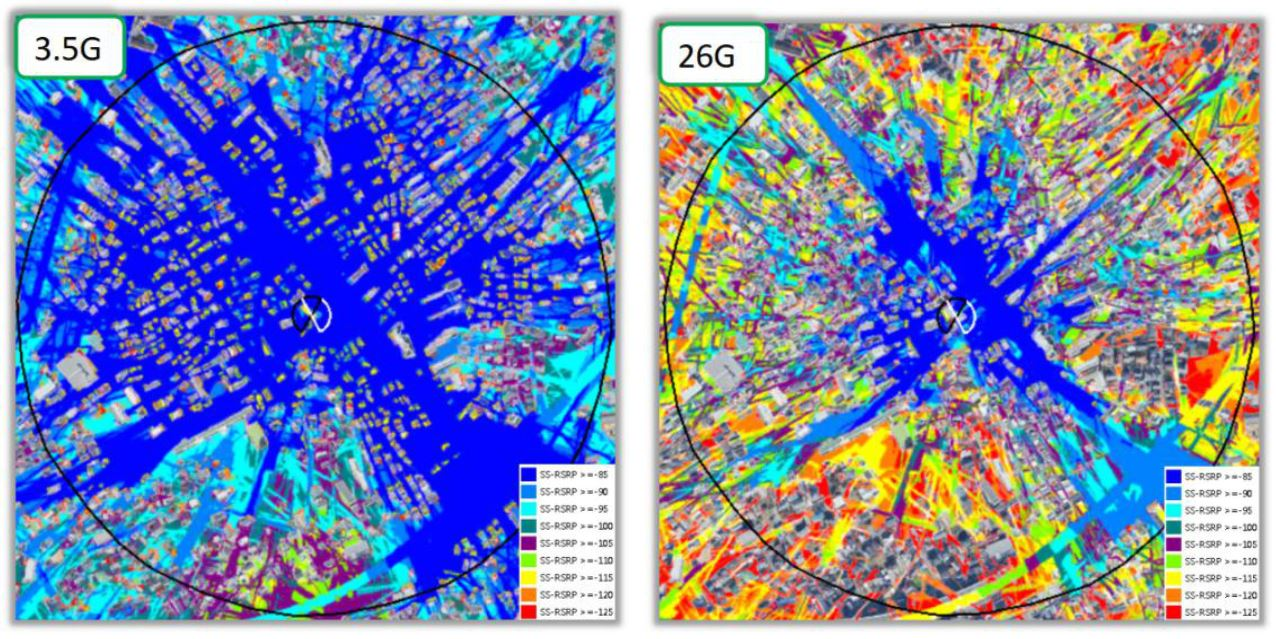
\includegraphics[width=0.8\linewidth]{Figures/Overlay-comparison.JPG}
\end{generalfig}

从毫米波设备的硬件架构来看,毫米波设备由大量的射频链路、射频开关、移相器组成用来实现模拟波束赋形。这样的收发器的组成需要所需的天线、放大器等器件相比现有通信方案增加多达数十倍,造成了成本长时间居高不下。
同时带来的也有能耗问题,复杂的射频硬件电路带来了令人难以置信的高功耗,这不是绿色通信的发展方向,也不利于实现碳中和(carbon neutrality)。

面对这些问题,急需一种能够规避高频信道的不可靠性的方法,其中重要的一环便是改善当前的无线环境。
中继站是一种可以将非视距路径(Non-line-of-sight, NLoS)转化为视距路径的方法\cite{Dohler2010a}。
使用中继站传输时,需要为每个中继站配备专用的电源和射频前端,这需要很高的资本投入,而且,中继站需要先接收处理无线信号再做转发,会带来较大的时延,更为严重的是,广播出的新信号可能会干扰原有信号\cite{di2020reconfigurable}。
反射阵列给出了有效的解决方案:当LoS径不能提供服务时,另一种建立替代路径的方法是通过无源非可重构镜面反射器,例如介质镜等。
反射阵列是指能够以波束的形式反射电磁波的平面\cite{huang2005reflectarray},这和曲面的反射镜不同,后者依靠物理曲率的变化决定反射波束的方向,而前者是由离散的单元组成,每个单元对应着不同的幅度和相移\cite{pozar1997design}。
无源非可重构的反射器与传统中继器相比,在成本和功耗方面有一定的优势。
但是,这种反射器的一个重大缺陷是它的反射在生产制造出来后就被固定了,在部署和使用是不可以修改,这无法适应高动态的无线信道环境。

近年来,人们研制出了能够对撞击的无线电波进行特定变换的基于电磁的可重构结构,它们的工作频段非常广阔,可以覆盖Sub-6 GHz、毫米波甚至太赫兹\cite{Wu2019}。下面一小节将详细介绍这一新技术。

\subsection{智能超表面概述}

它们被称为可重构智能表面(RiS),当部署在无线网络中时,有可能将无线环境(本质上是高度概率性的)转变为可编程和部分确定性的空间,称为智能无线电环境[5]。本文的目的是介绍这一主题,重点是与继电器辅助系统的区别。

\subsection{国内外现状分析}
智能超表面(也被称为智能反射面)的主要组成部分是可编程人工电磁表面结构。该结构是
一种由精心设计的亚波长单元按照周期或非周期性的排列组成的,具有可重配电磁特性的二
维薄层。基本单元通常由金属、介质和可调器件构成。通过控制反射单元的可调部分,例如
电磁波的幅度、相位,能够实现对电磁波传播方向的调控。该技术是近两年刚刚兴起的国际
学术界研究热点。然而目前国内外绝大多数的研究只停留在理论分析与建模仿真阶段,基于
智能超表面的无线通信实验验证系统十分稀缺。
多伦多大学实现了一个6×6 可重构发射天线阵列,每个振子连接一个变容二极管以增强其波
束扫描角度范围。在5 GHz频率下,实现了100×100度的扫描窗口范围。中国科学院光电技术
研究所研究团队通过变容二极管和PIN二极管实现了在微波波段(13.5 GHz以内)对电磁波多
个维度的控制,包括波束分裂、波束偏转、偏振变换等功能。东南大学崔铁军院士团队中提
出了一种同时在时间和频率上操纵电磁波的时空调制数字可编程超表面。以上研究主要关注
电磁超材料的设计本身,并没有在智能超表面对移动通信的增强上做过多研究。
与无线通信相关的智能超表面硬件演示系统方面。东南大学团队提出了基于二进制频移键控
的超表面,并通过数字编码序列控制离散反射相位,另外还设计了一个基于可编程表面的正
交相移键控(QPSK)无线发射机的原型。这两个原型系统是通过智能超表面实现信号的编码
与调制,本质上属于一种信号源,与本团队的作品差别较大。2019年MIT研究团队展示了一个
由3000多个无源天线组成的反射面(由几十个PCB板拼接而成),工作频率为1.6 GHz-3
GHz。实验表明它可以使接收信号强度增加10倍,将信道容量提升两倍。2019年清华大学研究
团队最近展示了一个工作在毫米波波段的16×16单元的智能超表面。可实现两比特的反射相
位调整。这个系统实现了28.5 GHz下19.1 dBi的天线增益。然而该系统的设计初衷是与喇叭
天线结合使用,替代传统的相控阵天线,与本团队的作品在设计理念和使用场景上有本质区
别。
本团队近期自主开发完成由1100个单元组成的智能超表面原型样机。团队在华中科技大学校
园内进行了室外空口性能测试,测得接收信号强度提升500倍,实现了500米远距离传输测
试,在智能超表面辅助下实现了高清视频的实时播放。

\subsection{本文主要研究内容与组织结构安排}

本文的主要研究内容是如何利用可编程电磁超表面增强 5 GHz WiFi的覆盖。文中 设计 了 一 个由 可编程超表面及其控制电路 构成的智能反射面系统 然后 将 它

招商银行股份有限公司

\section{相关理论}

\subsection{啊这,不知道有什么原理呢。}

\subsection{波束赋形}
\section{仿真分析}
\section{系统设计}

这个系统怎么设计呢?\footnote{哈哈哈}


\subsection{saasd}

\section{实验数据}
\section{总结与展望}
\section{段落}
\paragraph{段落}\label{para:para}这是一个带有顶头标签的段落这是一个带有顶头标签的段落这是一个带有顶头标签的段落这是一个带有顶头标签的段落这是一个带有顶头标签的段落这是一个带有顶头标签的段落这是一个带有顶头标签的段落
\subparagraph{小段落}\label{subpara:subpara}只是一个带有缩进标签的段落只是一个带有缩进标签的段落只是一个带有缩进标签的段落只是一个带有缩进标签的段落只是一个带有缩进标签的段落只是一个带有缩进标签的段落只是一个带有缩进标签的段落
\subsection{第二小节}
本模板已经引入伪加粗和伪斜体,这样就不需要对应的粗体和斜体字体也能生成需要的效果,就像下面这样

{\songti \bfseries 宋体加粗}

{\songti \itshape 宋体斜体}

{\songti \bfseries \itshape 宋体粗斜体}

请注意,使用加粗和斜体时,请与字体名称一同使用,否则会自动将粗体匹配为黑体,斜体匹配为楷体,就像下面这样

{正常显示宋体}

{\bfseries 加粗后变为黑体}

{\itshape 斜体后变为楷体}

\subsection{第三小节}

\begin{algorithm}
	\caption{Greedy Fast Beamforming Algorithm}
	\label{alg:GreedyAlgorithm}
	\begin{algorithmic}[1]
		\STATE \textbf{Input: } The feedback of RX signal power $p_t$.
		\STATE \textbf{Output: } The reflection coefficients matrix.
		\STATE Initialize a reflection coefficients matrix $ \mathbf{R}_0\in \mathbb{C}^{M \times N }$;
		\STATE Receive initial feedback of the RX signal power $ p_0 $;

		\STATE // Horizontal search;
		\FOR {each $n \in [1, N]$}
		\STATE  $ \mathbf{R}_{n} \leftarrow [\mathbf{r}_{n-1,1},\cdots,\mathbf{r}_{n-1,n-1},- \mathbf{r}_{n-1,n}, \mathbf{r}_{n-1,n+1}\cdots,\mathbf{r}_{n-1,N}] $;
		\STATE Receive feedback $ p_{n} $ using configuration $ \mathbf{R}_{n}$;
		\IF {$ p_{n-1} \ge p_{n}$}
		\STATE $ \mathbf{R}_{n} \leftarrow \mathbf{R}_{n-1}$;
		\ENDIF
		\ENDFOR
		\RETURN{reflection coefficients matrix $ \mathbf{R}_{N}$;}

		\STATE // Vertical search;
		\STATE Denote $ \mathbf{R}_{N} =[\mathbf{s}_{N,1},\mathbf{s}_{N,2},\cdots,\mathbf{s}_{N,M}]^\mathrm{T}$;
		\FOR {each $m \in [1, M]$}
		\small
		\STATE  $\mathbf{R}_{N+m} \leftarrow [\mathbf{s}_{N+m-1,1},\cdots,\mathbf{s}_{N+m-1,m-1},- \mathbf{s}_{N+m-1,m}, \mathbf{s}_{N+m-1,m+1}, \cdots, \mathbf{s}_{N+m-1,M}]^\mathrm{T}$;
		\normalsize
		\STATE Receive feedback $ p_{N+m} $ using configuration $\mathbf{R}_{N+m}$;
		\IF {$ p_{N+m-1} \ge p_{N+m}$}
		\STATE $ \mathbf{R}_{N+m} \leftarrow \mathbf{R}_{N+m-1}$;
		\ENDIF
		\ENDFOR
		\RETURN{reflection coefficient matrix $ \mathbf{R}_{M+N}$.}
	\end{algorithmic}
\end{algorithm}









\section{参考文献和交叉引用}\label{sec:ref}
\subsection{参考文献}
这是一个参考文献引用的范例\cite{9326394, Renzo2019,5502350, liang2019large, CHN_zhou2020, CHN_zhang2017}




\subsection{交叉引用}\label{subsec:crossref}
本模板已经重写了hyperref宏包的\verb|\autoref|命令,方便引用章节、公式和图表。

比如说\autoref{sec:ref}和\autoref{subsec:crossref}就引用了本章节,\autoref{para:para}和\autoref{subpara:subpara}引用了之前的两个段落。显然段落因为没有序号,引用结果和上一节的需要相同,因此建议使用段落“\nameref{para:para}”和段落“\nameref{subpara:subpara}”。

\section{公式这么用}
在文中引用公式可以这么写:$a^2+b^2=c^2$这是勾股定理,他还可以表示为$c=\sqrt{a^2+b^2}$,还可以让公式单独一段并且加上编号
\begin{equation}
	\sin^2{\theta}+\cos^2{\theta}=1 \label{eq:pingfanghe}
\end{equation}
还可以通过添加标签在正文中引用公式,如式~\eqref{eq:pingfanghe}~或者\autoref{eq:pingfanghe}。我们还可以轻松打出一个矩阵
\begin{equation}
	\bm{A}=\begin{bmatrix}
		1  & 2  & 3  & 4  \\
		11 & 22 & 33 & 44 \\
	\end{bmatrix}
	\times\begin{bmatrix}
		22 & 24 \\
		32 & 34 \\
		42 & 44 \\
		52 & 54 \\
	\end{bmatrix}
\end{equation}
或者多个带编号的公式
\begin{eqnarray}
	f_1(x)=12x^2+36x+\sin x\\
	f_2(x)=\sqrt{3}{x^3+3x}
\end{eqnarray}
以上

\section{用图和表的示例}
\subsection{图的使用}
\XeLaTeX 环境下可以使用EPS、PDF、PNG、JPEG、BMP格式的图片,当然也可以用绘图包直接在\LaTeX 中绘制图形,推荐使用宏包tikz。图的环境是figure,但figure环境使用复杂且不自带标题,因此本模板定义了一个通用版本的generalfig,该环境会将figure内的图片居中并设置标签与引用名,同时会让图片位置设置为所有可行位置(htbp,即此处、页顶、页底、独立一页),此选项可以作为可选参数设置。

其使用方法如下:\autoref{fig:50mcopper}


\autoref{fig:50mtest}

\ref{fig:50mcopper}

\ref{fig:50mtest}

\begin{figure}[t!]
	\centering
	\subfloat[df哈哈]{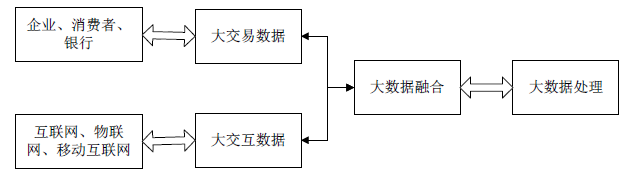
\includegraphics[width=0.5\linewidth]{Figures/data.png}%
		\label{fig:50mphoto}}
	\hfil
	\subfloat[dd]{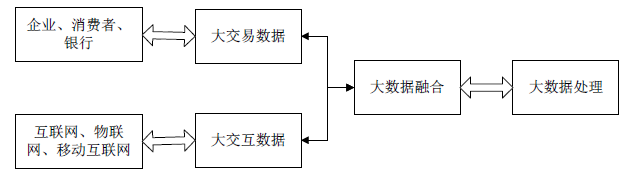
\includegraphics[width=0.5\linewidth]{Figures/data.png}%
		\label{fig:copper}}
	\hfil
	\subfloat[fs]{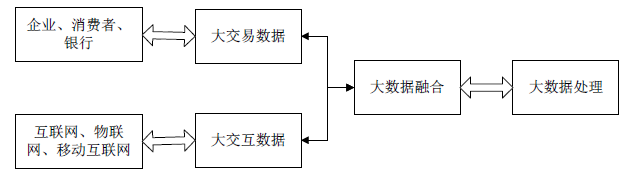
\includegraphics[width=0.5\linewidth]{Figures/data.png}%
		\label{fig:50mgreedy}}
	\hfil
	\subfloat[dfdf]{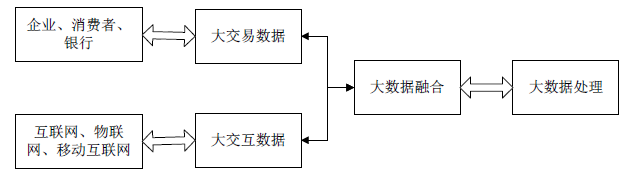
\includegraphics[width=0.5\linewidth]{Figures/data.png}%
		\label{fig:50mcopper}}
	\caption{The 50 m outdoor over-the-air test: (a) the scene of the transmitter and receiver; (b) a copper plate of the same size as the RIS; (c) spectrum when using the RIS; (d) spectrum when using the copper plate.}
	\label{fig:50mtest}
\end{figure}

\begin{figure}[htb]
	\centering
	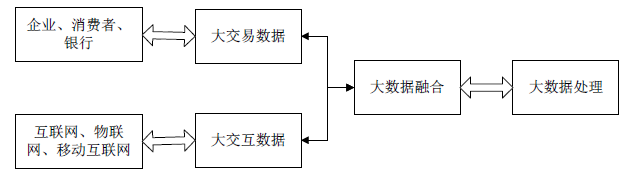
\includegraphics[width=0.5\linewidth]{Figures/data.png}
	\caption{Indoor non-LoS test.}
	\label{fig:through_wall}
\end{figure}

\begin{generalfig}[htb]{大数据信息处理框架}{fig:data}
	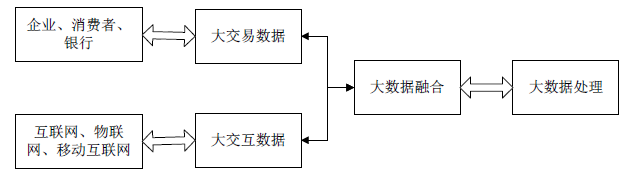
\includegraphics[width=0.4\linewidth]{Figures/data.png}
\end{generalfig}

同时也可以引用该图片例如:\autoref{fig:data}或者图~\ref{fig:data}。请注意generalfig第一个参数是标题,第二个参数是引用。

\newpage

\subsection{表的使用}
作为论文,推荐使用三线表进行排版。所谓三线表,即在标题前有横线,标题后有横线,表格最后还有横线,其他地方无线。当然这不是死规定,也可以根据需要在合适的地方加线。
、踩踩踩
本文定义了新的可变长度左中右(LCR)格式,LCR三个格式会根据表格宽度的设定自行控制宽度,且其宽度相等,方便设置和页面相同宽度的表格。但该功能需要使用tabularx做表。
\begin{generaltab}{某校学生升高体重样本}{tab:heightweight}
	\begin{tabularx}{\textwidth}{lCCC}
		\toprule
		序号 & 年龄 & 身高   & 体重  \\ \midrule
		1    & 14   & 156    & 42    \\
		2    & 16   & 158    & 45    \\
		3    & 14   & 162    & 48    \\
		4    & 15   & 163    & 50    \\
		\cmidrule{2-4} %添加2-4列的中线
		平均 & 15   & 159.75 & 46.25 \\ \bottomrule
	\end{tabularx}
\end{generaltab}

当然你也可以引用表格,就像这样:\autoref{tab:heightweight}。

\section{列表的使用}
这是一个计数的列表
\begin{enumerate}
	\item 第一项
	      \begin{enumerate}
		      \item 第一项中的第一项
		      \item 第一项中的第二项
	      \end{enumerate}
	\item 第二项
	\item 第三项
\end{enumerate}

这是一个不计数的列表
\begin{itemize}
	\item 第一项
	      \begin{itemize}
		      \item 第一项中的第一项
		      \item 第一项中的第二项
	      \end{itemize}
	\item 第二项
	\item 第三项
\end{itemize}

\begin{thankpage}
	
	{\itshape “文章本天成,妙手偶得之。”}

	{\itshape “朝发鸡鸣未响,归路晚风凉。汗洒澄池桃李,几度银杏黄。”}

	\begin{figure}[htb]
		\flushright
		
\includegraphics[width=15mm]{Figures/Seal-pxl.pdf}
	\end{figure}

	\begin{flushright}
		2021年5月10日

		于华中科技大学韵苑
	\end{flushright}
	
\end{thankpage}

%生成参考文献
%使用方法:\bibliography{参考文件1文件名, 参考文献2文件名, ...}
\bibliography{Bibs/references_Gradu}

\begin{appendices}
	\section{系统电路原理图}
	\section{这是第一个附录}
	这里是附录环境,其中的section、subsection、subsubsection已经变为附录的样式,并且会以这种样式加入目录中。
	\subsection{附录可以有小节}
	\subsubsection{附录中也可以有小小节}\label{apxsubsubsec:appendix}
	\subsubsubsection{附录中也有小小小节}
	\verb|\autoref|无法识别Appendices环境,引用效果和正文一样,如\autoref{apxsubsubsec:appendix}。所以如果引用附录的话,建议直接使用附录~\ref{apxsubsubsec:appendix}。
\end{appendices}

\end{document}




